\newpage
\section{Introduction}
\subsection{Savanna distribution}

Tropical savannas dominate the seasonally dry tropical climatic range across Africa, Australia, South America and parts of South East Asia \citep{murpheyetal2015}. Covering between $20\%$ \citep{murpheyetal2015, williamsetal1997} to 25\% \citep{collinsetal2009} of the worlds terrestrial landscape. Within Australia, tropical savanna occupies approximately one quarter of the continent, across the northern part of Queensland (QLD), the Northern Territory (NT) and Western Australia \citep{foxetal2001}.

Tropical savanna is the dominant vegetation class within the northern third of the NT \citep{houseHall2001}. The primary constraints for tropical savannas, woodlands and grasslands distribution is rainfall and seasonality \citep{foxetal2001, houseHall2001}. Dominating the north, where annual rainfall is between $500$ mm and $1800$ mm per year (Figure \ref{fig:rainfall}) \citep{williamsetal1997}. Where $90\%$ of rainfall occurs between November and April (wet season) with the remaining $10\%$ of rainfall occurring between May and October (dry season); causing sufficient water stress that many woody vegetation forms shed their leaves, and grasses cure \citep{williamsetal1997}.

\begin{figure}[h]
\centering
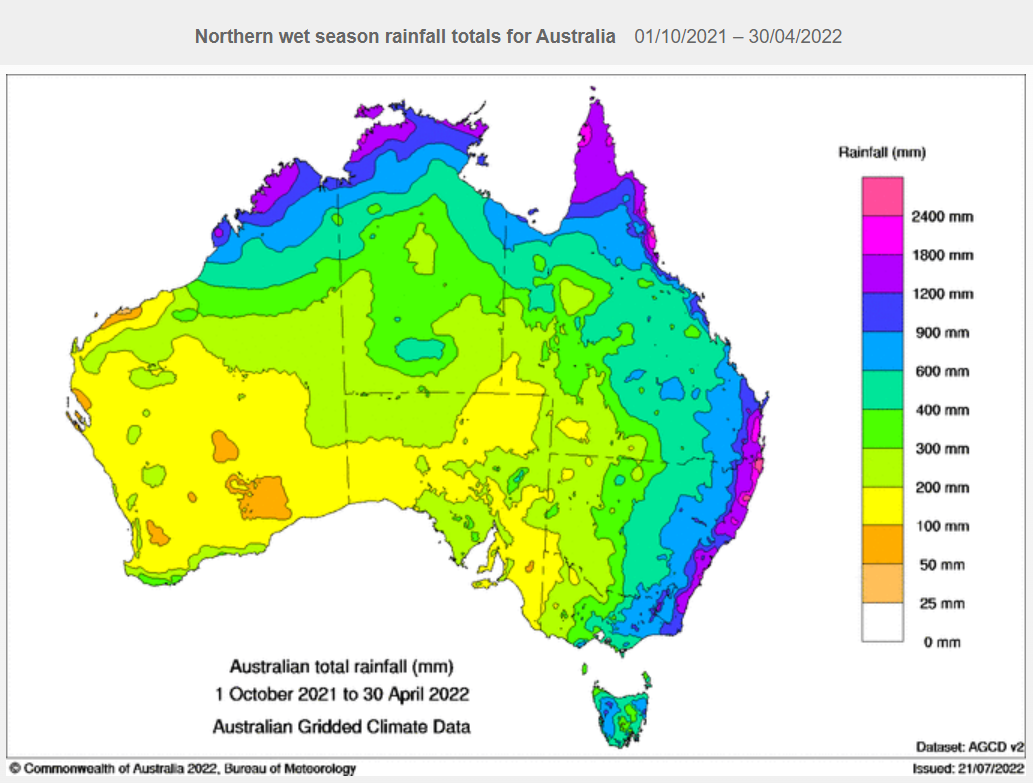
\includegraphics[scale=0.3]{images/bom_2022_wet_season.png}
\caption{Annual rainfall between October 2021 and April 2022.}
\label{fig:rainfall}
\end{figure}
\citep{bom2022}

\subsection{Variability of savanna}
Although the vegetation class of tropical savanna may appear homogeneous within the NT, there is significant variability within its distribution. Tropical savanna is defined as an open woody upper stratum over persistent c4 grasses \citep{williamsetal1997}, with or without a mid stratum of woody shrubs \citep{lehmannetal2011}. The savanna vegetation class of the NT, consists of tall eucalypt dominated woodlands or open woodlands in the coastal and sub-coastal regions, transitioning into low Acacia dominated shrublands, and almost treeless grasslands towards the semi arid southern part of its distribution \citep{foxetal2001, williamsetal1997, woinarski2007}; following  the NT's rainfall gradient \citep{houseHall2001, hutleyetal2011, lehmannetal2011, williams1996}.

In addition to rainfall, soil nutrients affect savanna variability and contribute to patchiness \citep{williams1996}. According to \cite{houseHall2001} low soil fertility within low rainfall regions will generally transition savanna from a semi-arid to an arid vegetation class. Conversely, high soil fertility within high rainfall regions will generally transition savanna woodland into forest \citep{houseHall2001, williams1996}. Therefore, soil variability in conjunction with rainfall increases savanna variability and patchiness within the NT.

In recent decades more emphasis has been placed on fire than climate and/or soil nutrients as a driver of savanna distribution and variability. According to \cite{prioretal2010}, savanna tree recruitment is thought to be subject to a fire-mediated bottleneck, where frequent fire inhibits the transition of a sapling into a mature tree. However, this model was derived from African savanna research, and \cite{murpheyetal2015} disputes the effectiveness of this model within an Australian context. Further stating, that eucalypt dominated Australian savannas avoid the fire trap as their extreme fire tolerance makes them relatively unresponsive to fire, reaching fire resistant size more quickly than other trees \citep{murpheyetal2015}.

Further to this, fire generally acts as a positive feedback, reducing canopy cover, thereby increasing c4 grass production \citep{bondetal2005, bond2008, woinarskietal2004b}, which increases fuel loads and may result in higher fire intensity \citep{lehmannetal2011, ratnametal2011}. Additionally, studies have demonstrated that savanna has transitioned into forest with the removal of fire on multiple continents \citep{bond2008}, including Australia \citep{woinarskietal2004b}. Further to this, fire is known to reduce tree growth and diameter at breast height (DBH) in northern Australian savannas \citep{murphyetal2010, williams1999}, and increase the size of tree hollows which result in less above ground biomass (AGB) \citep{peetersbutler2014}. 

\subsection{Carbon storage}
Due to the global distribution of tropical savannas, they are considered an important carbon (C) sink. According to \cite{Graceetal2006} on average, global savannas store $\sim120 \ tC \ ha^{-1}$ within its vegetation mass and organic soil matter. Although this is less than half that of global tropical forest ($\sim320 \ tC \ ha^{-1}$), it still represents $\sim15 \%$ of global stored C \citep{Graceetal2006}. Within northern Australian tropical savanna, C stock has been measured at $\sim53 \ tC \ ha^{-1}$ \citep{chenetal2002}, which is less than half that of the global average. Even though the two biomes record a similar net primary production NPP, the difference in C stock is primarily the result of frequent fires; returning sequestered C back into the atmosphere \citep{Graceetal2006}. Therefore, even though global and northern Australian tropical savanna store less C than tropical forests, due to their distribution they are still an important C sink.

\subsection{Emissions from land clearing}
Australian tropical savannas (including the NT) remains structurally intact from agriculture and land use change \citep{franklinetal2008, hutleyetal2016, kuttetal2012}. Since clearing controls began in 1999 for zoned and unzoned land tenure \citep{ntplanningact1999}, and 1992 for pastoral lease tenure \citep{ntpastorallandact1992} within the NT; $\sim1974\ km^2$ of tropical savanna has been approved for clearing \citep{unzonedclearing2022, pastoralclearing2022}. Additionally, according to land use mapping undertaken by \cite{landuse2016}, $\sim4563 \ km^2$ of what once was likely considered tropical savanna has undergone land use change or deforestation for agriculture and intense use. However, the total amount of clearing (full felling and selective clearing) within the NT is unknown.

According to \cite{hutleyetal2016}, the total emissions released from clearing native savanna woodland for a site located $\sim300 \ km$ south of Darwin, equated to $148.3 \ Mg\ CO_{2}-e \ ha^{-1}$. Of the total emissions, $82\%$ was released due to the burning of biomass, $10\%$ were attributed to soil disturbance and $8\%$ attributed to debris curing and decay.

\subsection{Quantifying AGB and C extent at a regional scale}
Understanding C sinks and sources within the tropical savanna context is necessary for decision makers and C accounting. However, accurately quantifying C emissions from land use change and fire at a local or regional level is difficult due to lack of existing baseline data \citep{woinarski2007}, financial constraints and structural variability \citep{barrettetal2001, houseHall2001}. Although the NT has a significant store of vegetation, fire scar, land system spatial data, and many remotely sensed products, the NT does not have regional scale AGB mapping.

\subsection{Estimating AGB}
AGB is an important biophysical parameter for understanding the C cycle within a terrestrial context. The most accurate way to estimate biomass is through direct measurements; however, this method is destructive and requires the termination of the tree \citep{clarkkellner2012, luetal2014}. Nonetheless, direct measurements of AGB, often result in the development of allometric models \citep{clarkkellner2012, luetal2014}. Once allometric models have been developed for a region, or vegetation community, stand biomass can be estimated using diameter at breast height (DBH) or DBH in conjunction with tree height biophysical parameters \citep{cooketal2005, williamsetal2005b}, which is non-destructive and data collection is less prohibitive \citep{clarkkellner2012, luetal2014}. However, it is important to note that estimating stand biomass from allometric models may lead to significant uncertainty, due to the fact that soil conditions, rainfall gradients, tree density and land-use history all influence growth rates, which effect tree height and DBH, and therefore estimated AGB (EAGB) \citep{clarkkellner2012}.

\subsection{Scaling up EAGB}
Nonetheless, there are many examples of modeling EAGB from satellite derived surface reflectance (SR) and other modeled products throughout the world \citep{gasparretal2010, lietal2020, wuetal2016, wuetal2022, zhengetal2004}. 
Whereby EAGB (from allometric scaling) is scaled up to remotely sensed data; as only airborne or satellite derived data allows the ability to sample large areas of the required vegetation class or biome \citep{clarkkellner2012}. However, extrapolating relationships between EAGB values with the spectral signatures of SR bands, spectral indices (SI) and/or modeled biophysical vegetation parameters, adds error into the predictions \citep{clarkkellner2012}. Accordingly, it is important to assess the model for accuracy and precision \citep{clarkkellner2012}.

According to \cite{clarkkellner2012}, the distinction between the accuracy and precision of modeled EABG at a regional scale derived from field based EAGB and satellite data is critical. Nonetheless, depending on its use, remotely sensed metrics with unknown accuracy are arguably sufficient for monitoring EAGB and EC stocks within a land type, and therefore, approximate loss of EABG and EC from historic and future land clearing at a regional level. Additionally, such a product could arguably be useful in the monitoring of long term trends in EAGB resulting from burning practice. However, such a product would not contain sufficient accuracy to report on global C accounting budgets or to inform $CO^2$ equivalent emissions for scientific climate change research \citep{clarkkellner2012, wuetal2016}.